\chapter{Literature Review}
\label{sec-literature-rev}

Within the research field of organizational and development economics, the paper by \cite{Ubfal2022} focuses on whether business training programs in developing countries can provide entrepreneurs with the skills they need to improve their business outcomes. To address this question, the assumptions behind these programs and their designs have changed over the years, for instance, with the inclusion of psychological insights. Several papers report positive treatment effects of teaching either technical or soft skills, while others find heterogeneous or no significant effects. In this Section, a few related papers to \cite{Ubfal2022} are presented.

\section{The Standard Approach}

Researchers began studying the power of business training programs when their contents were still revolving around practical (hard) skills, such as quality management, record keeping, and business planning.

For instance, \cite{Mano2012}, in "How Can Micro and Small Enterprises in Sub-Saharan Africa Become More Productive?", performed an RCT in Ghana on 167 entrepreneurs to examine the effects on their survival rate, profits, and adoption of recommended business practices. The treatment consisted of classes based on materials from the International Labour Organization (ILO), such as Start Your Business (SYB) and Improve Your Business (IYB). After one year, their findings revealed a higher survival rate and wider adoption of recommended business practices, however, they found feeble positive effects on profits. Similarly, in "Less is More: Experimental Evidence on Heuristic-Based Business Training in Ecuador", \cite{Arraiz2019} revealed the lower influence on profits of traditional business training to alternative (heuristic) approaches. In a meta-analysis, \cite{McKenzie2020} gathers the results of a number of studies, finding an average increase of 5-10\% in entrepreneurs' profits after standard business training.

Such a small influence on profits made researchers question about the cost-benefit of these programs and what could be improved in their design to boost their impact. Therefore, a number of proposals and innovations for these trainings have arisen, among others, kaizen methods, mentoring, heuristics, and psychology insights. \cite{McKenzie2020} presents the results of these alternative approaches and highlights their greater power in positively influencing entrepreneurs' profits, by an average of 14\%.
\begin{figure}[t]
    \centering
    \caption{Estimates of the Impact of "Standard" (left) vs "Alternative" (right) Business Training on Firm Profits (extract), \cite{McKenzie2020}}
    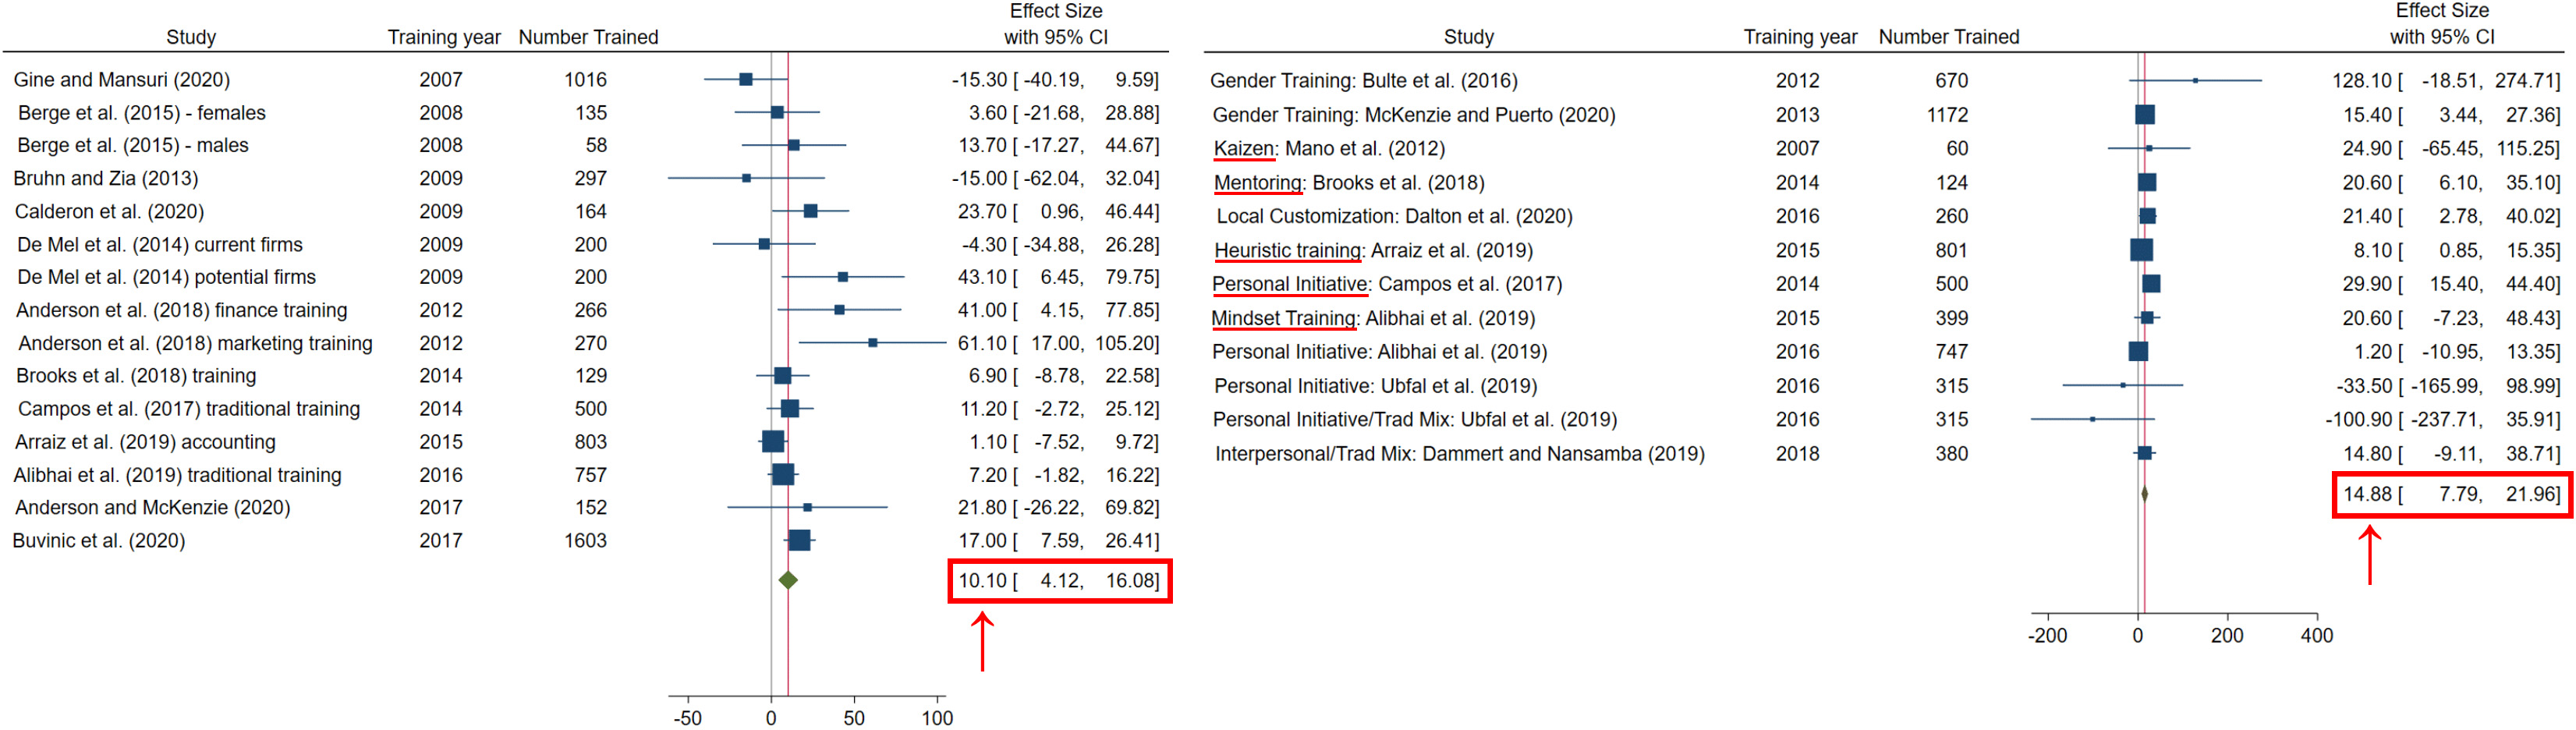
\includegraphics[width=\textwidth]{img/meta-analysis.jpg}
    \label{meta-analysis}
\end{figure}

\section{Including Psychology}

The extensions for the business training programs including psychological insights play an important role and are reviewed by \cite{Frese2014} in "The Psychology of Entrepreneurship". The authors define entrepreneurship as the process of identification and exploitation of business opportunities. A proactive personality drives business success and setting challenging goals yields higher performance over time. Furthermore, they discuss that personal initiative is pivotal throughout the entrepreneurial journey because it helps differentiate the business, create advantages, and achieve better results. Nevertheless, a persistent behavior and a critical and problem-solving attitude are intrinsic to a resilient business.  

All these characteristics can fall under the notion of soft-skills. Researchers have tested whether teaching soft-skills to entrepreneurs can actually improve treatment effects and, if so, through which channels. This is where the work of \cite{Ubfal2022} presented earlier comes in. In their study, they found that entrepreneurs in the soft skills group were more likely (11\%) to experience positive profits than those in combined training (7\%). Although they found that the increase in profits was mainly experienced by men, this change was due to greater adoption of recommended business practices by both men and women. In a similar study, "Teaching personal initiative beats traditional training in boosting small business in West Africa," \cite{Campos2017} demonstrated the effectiveness of such programs. In 2014, they conducted an RCT on 1,500 Togolese microenterprises. One treatment group received classical business training, while the other was taught lessons on developing a proactive entrepreneurial mindset. Similar to \cite{Ubfal2022}, the results supported the initial hypothesis that teaching entrepreneurs soft skills can better influence profits: over the time span of the experiment (2.5 years), monthly profits increased by 30 percent. In contrast to the results of \cite{Ubfal2022}, they found that this increase is experienced by both men and women, but confirmed the adoption of new recommended practices as the main intermediate mechanism. In addition, their results seem to be more persistent throughout the duration of the experiment, which could be due to the participants' monthly visits conducted by a trainer ready to answer any questions and help them implement the principles taught during the training.

\section{Including Mentors}

Another relevant extension to basic business training is the inclusion of mentors assisting the participants.

For instance, in "Business Training and Mentoring: Experimental Evidence from Women-Owned Microenterprises in Ethiopia" by \cite{Bakhtiar2022}, the authors test the effects of regular business training and mentoring for women-owned small firms in Ethiopia. Additionally, in response to the idea that it takes a while for changes in adopted business practices to translate into improved business outcomes, they examine the long-term impacts, up to 3 years after training. The RCT is structured as follows: first, the treatment group is given standard business training; second, the treated participants become mentors and are assigned three randomly selected mentees within their network. Mentors and mentees were asked to meet once a month for six months. While the first training significantly and positively affected participants' revenues and profits, the effects of mentoring on mentees' profits were positive but not significant. However, mentees experienced an increase in the adoption of business practices. In conclusion, \cite{Bakhtiar2022} mainly contributed to demonstrating the power of mentoring as a low-cost tool for transmitting knowledge and practices to improve business outcomes.
